\begin{figure}[H]
    \centering
    \begin{tikzpicture}[scale=1, every node/.style={font=\small}]

    \filldraw[fill=violet!30, opacity=0.2] (-2.5,0) rectangle (3,4); 
    \filldraw[fill=violet!60, opacity=0.4] (-2.5,-4) rectangle (3,0); 
    \filldraw[fill=blue!30, opacity=0.2] (3,0) rectangle (8.5,4); 
    \filldraw[fill=blue!60, opacity=0.4] (3,-4) rectangle (8.5,0);

    \node[rotate=90] at (-3,2) {Précurseurs (immature)};
    \node[rotate=90] at (-3,-2) {Cellules matures};
    \node at (0,4.3) {Myéloïde};
    \node at (6,4.3) {Lymphoïde};

    \node at (0,3.5) {\small \textbf{\gls{lam}}};
    \node at (6,3.5) {\small \textbf{\gls{lal}}};
    \node at (0,-0.5) {\small \textbf{\gls{smp}}};
    \node at (4.7,-0.5) {\small \textbf{\gls{slp}}};
    \node at (7,-0.5) {\small \textbf{\gls{lnh}}};

    \node at (0,1.7) {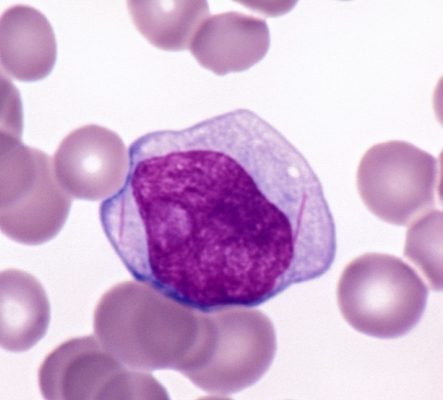
\includegraphics[width=3cm]{images/lam.jpg}};
    \node at (6,1.7) {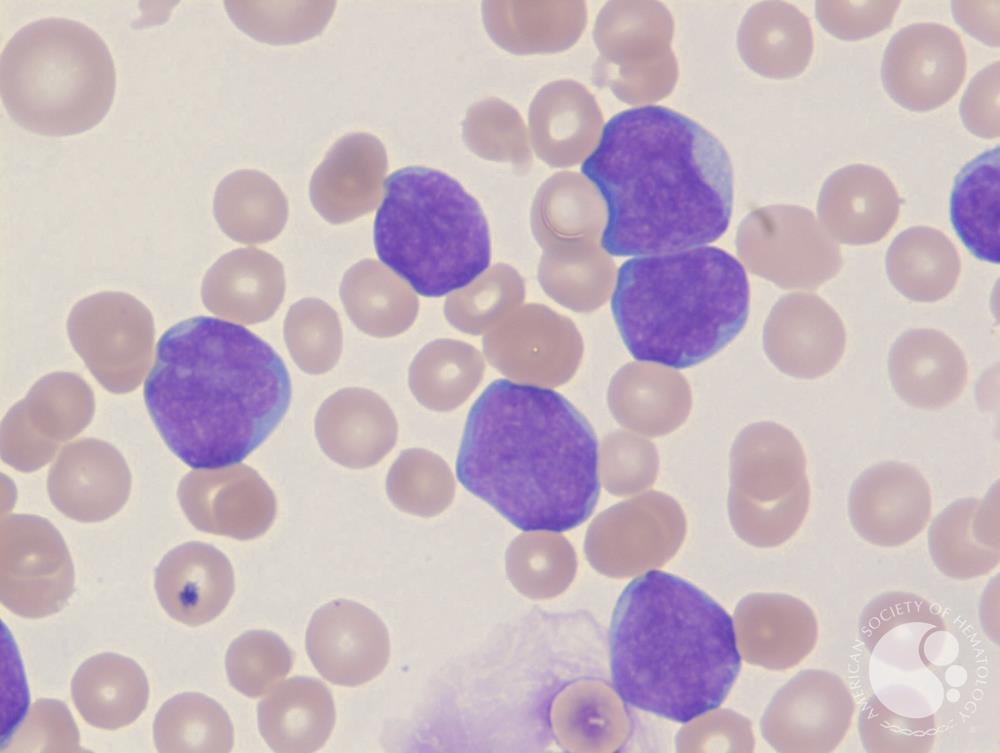
\includegraphics[width=3cm]{images/lal.jpeg}};
    \node at (-1,-2) {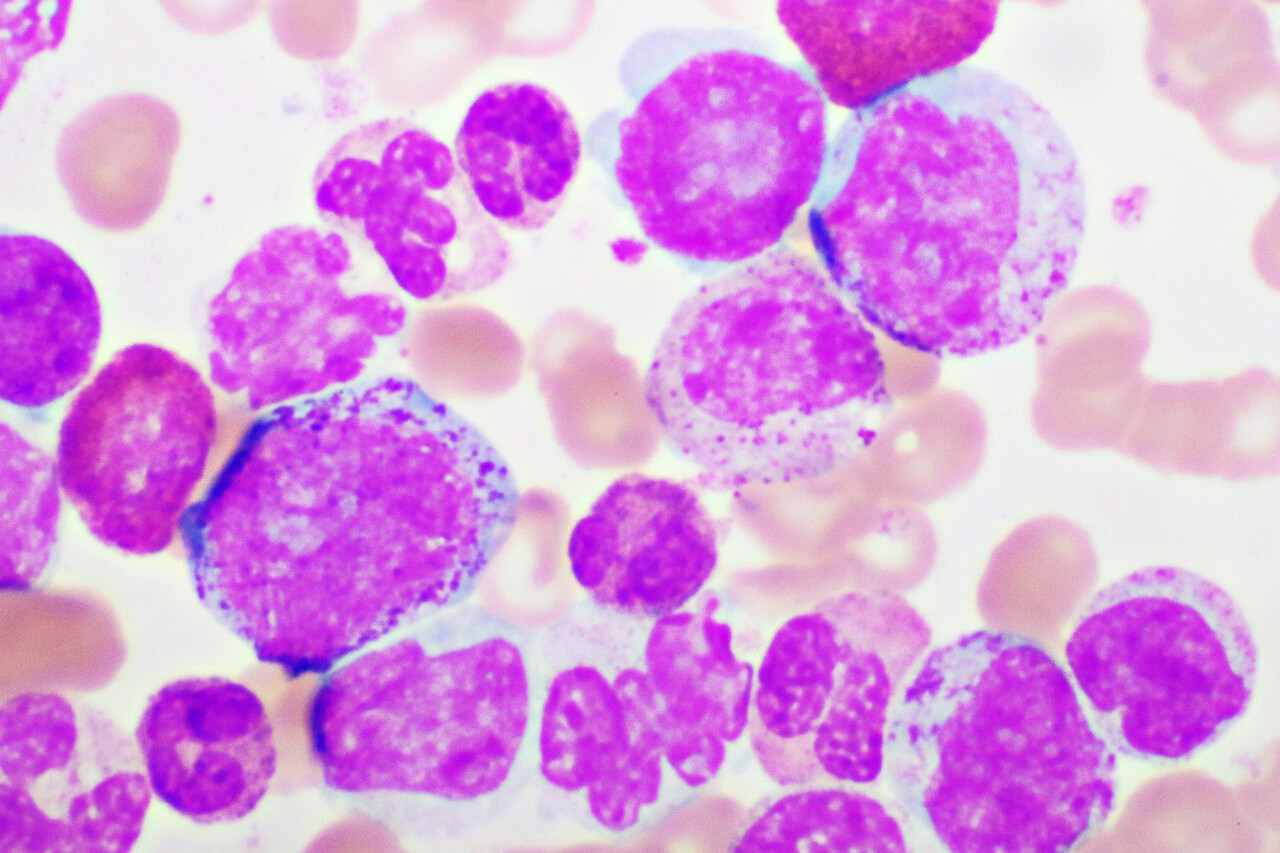
\includegraphics[width=2cm]{images/lmc.jpg}};
    \node at (1.2,-3) {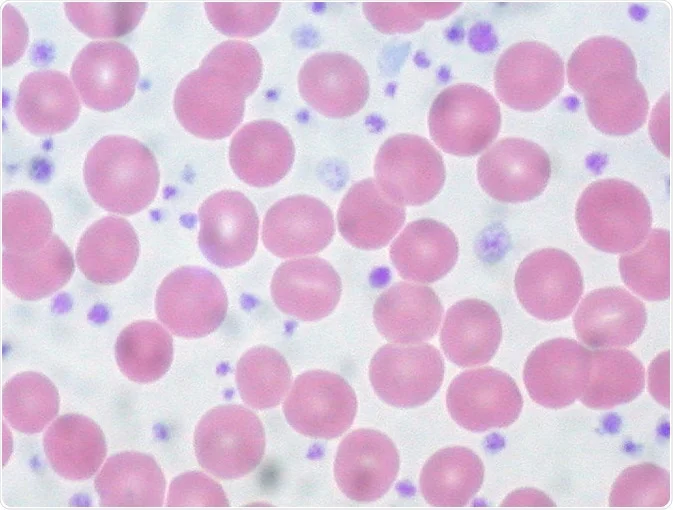
\includegraphics[width=2cm]{images/te.png}};
    \node at (4.7,-2) {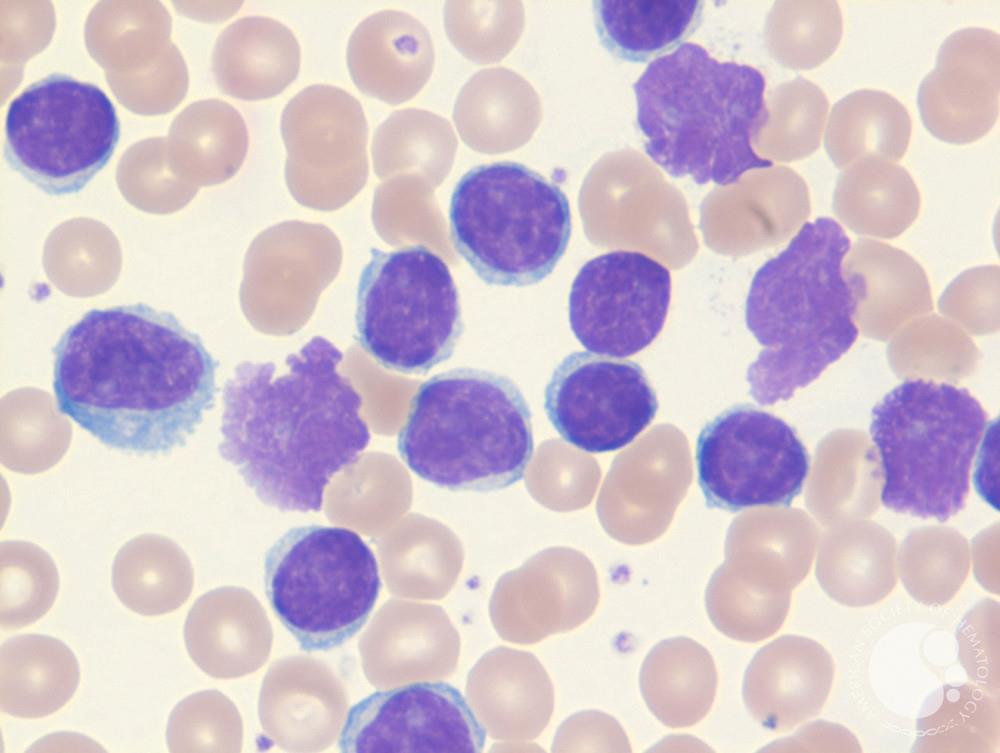
\includegraphics[width=2cm]{images/llc.jpeg}};
    \node at (7, -3) {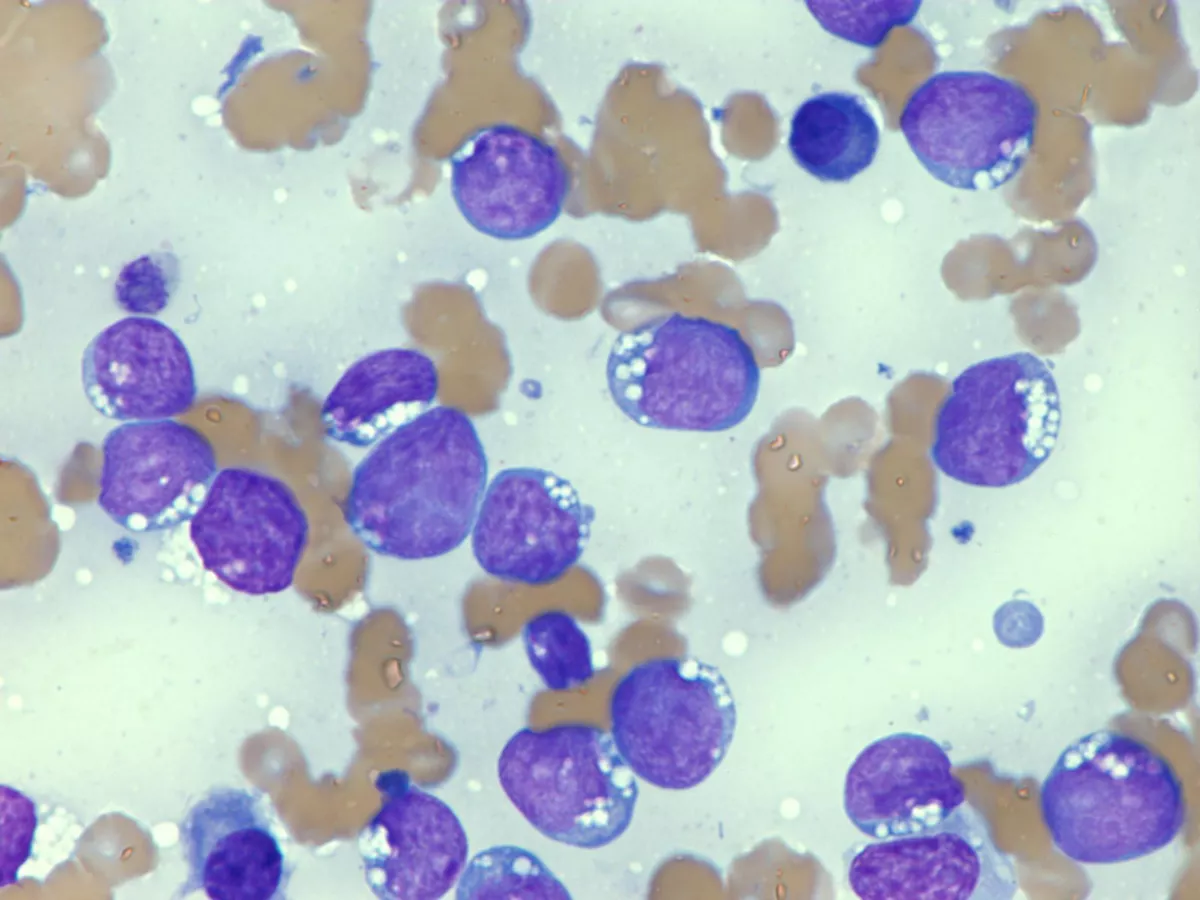
\includegraphics[width=2cm]{images/burkitt.png}};

    \draw[thick] (3,4.5) -- (3,-4.5); 
    \draw[thick] (-3,-0) -- (9,-0); 

    \end{tikzpicture}
    \caption{Classification des hémopathies malignes selon la lignée (myéloïde vs lymphoïde) 
    et le degré de maturité cellulaire (précurseur vs mature).}
    \label{fig:hemopathies}
\end{figure}
